\documentclass[10pt,a4paper]{article}

\usepackage[margin=1.05in]{geometry}
\usepackage{setspace,amsmath,amssymb,amsthm}
\usepackage{graphicx,enumitem,titlesec,fancyhdr,microtype}
\usepackage{hyperref}
\graphicspath{{../../drawings/pass2/}}
\hypersetup{colorlinks=true,linkcolor=black,urlcolor=black,citecolor=black}

\titleformat{\section}{\normalsize\bfseries}{}{0em}{}
\titleformat{\subsection}{\small\bfseries}{}{0em}{}
\titlespacing*{\section}{0pt}{1.35em}{0.5em}

\theoremstyle{plain}
\newtheorem{proposition}{Proposition}
\theoremstyle{definition}
\newtheorem{definition}{Definition}
\theoremstyle{remark}
\newtheorem{observation}{Observation}

\setstretch{1.14}
\pagestyle{fancy}
\fancyhf{}
\fancyhead[L]{\small\itshape Elements of Position}
\fancyhead[R]{\small\itshape I.\ The Closed Unit}
\fancyfoot[C]{\small\thepage}
\renewcommand{\headrulewidth}{0pt}

\begin{document}

\begin{center}
\vspace*{2.0em}
{\large Elements of Position}\\[1.5em]
{\LARGE\bfseries I.\ The Closed Unit}\\[2.0em]
{\normalsize Justin Erholtz}\\[0.3em]
{\small 12 September 2026}
\end{center}

\vspace{1.8em}

\begin{center}
{\large Where is \(1\)?}
\end{center}

\vspace{1.4em}

\noindent
Where is \(1\)? Point to it.

You cannot, and not because the mark is missing.
One is not an object on the table.
It is a finished hold --- the interior of which can be cut without end.
This work lives in that double fact: the unit closes, and the cut does not.

\vspace{1.0em}
\noindent
\textit{A note.}
A later part stands on this one.
It does not explain it.
Claims proved here are identities of a finished whole and of inversion through that whole.
A count, a kick, a residual, belong to later parts and are not imported.

\vspace{0.6em}
\noindent
\textit{A note on names.}
Closed unit --- \(1\), read as a finished whole.
Primary cut --- \(1/2\), the only self-equal split of the unit interval.
Pair --- \((n,1/n)\), product \(1\), geometric mean \(1\).
Lock --- the pair at \(n=1\), where the two places are one place.
Vacuum --- a relation named in one stroke.
Trace --- the same relation walked with cost.
The trace is Part~II.

\newpage
\tableofcontents
\newpage

\section{One}

Where is \(1\)?

It is an idea, and it is real in the abstract sense.
There is no specimen of which one can say \emph{that is one} and stop.
What there is, is one \emph{of} a thing: one stone, one step, one finished hold.
In its most basic sense one is not a specimen.
It is a closed object --- a unit that has completed itself.

That already splits.
Between \(0\) and \(1\) the cut can be repeated without end.
The interior of the unit is already endless; in that reading one never closes.
In the other reading one \emph{is} the close: the hold is finished, and that finished hold is what the word names.
Both readings are true of the same mark.
The work begins at that tension and does not dissolve it.

Infinity is already inside \((0,1)\).
It is not a later chapter and not a last tick.

\section{Two parts of a finished whole}

If a finished thing can still be cut, the first honest question is when the split is even.

\begin{proposition}
\label{prop:amgm}
For nonnegative \(a,b\),
\[
\frac{a+b}{2}\ge\sqrt{ab},
\]
with equality if and only if \(a=b\).
\end{proposition}

\begin{proof}
\(\bigl(\sqrt{a}-\sqrt{b}\bigr)^{2}\ge 0\) expands to \(a+b\ge 2\sqrt{ab}\).
Divide by \(2\).
\end{proof}

On the pair \((x,1-x)\) the arithmetic mean is constantly \(1/2\), and equals the geometric mean only at \(x=1/2\).
That is the only cut of the unit interval that is the same amount from both ends.
It is the primary cut.

On the pair \((x,2-x)\) the arithmetic mean is constantly \(1\), and equals the geometric mean only at \(x=1\).
The meeting value is \(1\), not \(1/2\): the whole being split is \(2\).

Inversion through the unit sends every positive mark to a partner whose product with it is still \(1\).

\begin{definition}[Pair]
For \(n>0\),
\[
r=n,\qquad \frac1r=\frac1n.
\]
\end{definition}

\begin{proposition}
\label{prop:pair}
\(r\cdot(1/r)=1\) and \(\mathrm{GM}(r,1/r)=1\).
\end{proposition}

\begin{proposition}
\label{prop:tau}
The leftover
\[
\tau(n)=\mathrm{AM}(n,1/n)-1=\frac{(n-1)^2}{2n}
\]
vanishes if and only if \(n=1\).
\end{proposition}

At \(n=1\) the pair is the lock.
The pair is \((1,1)\).
The leftover is \(0\).
The two places have not yet had room to differ.


\begin{figure}[htbp]
\centering
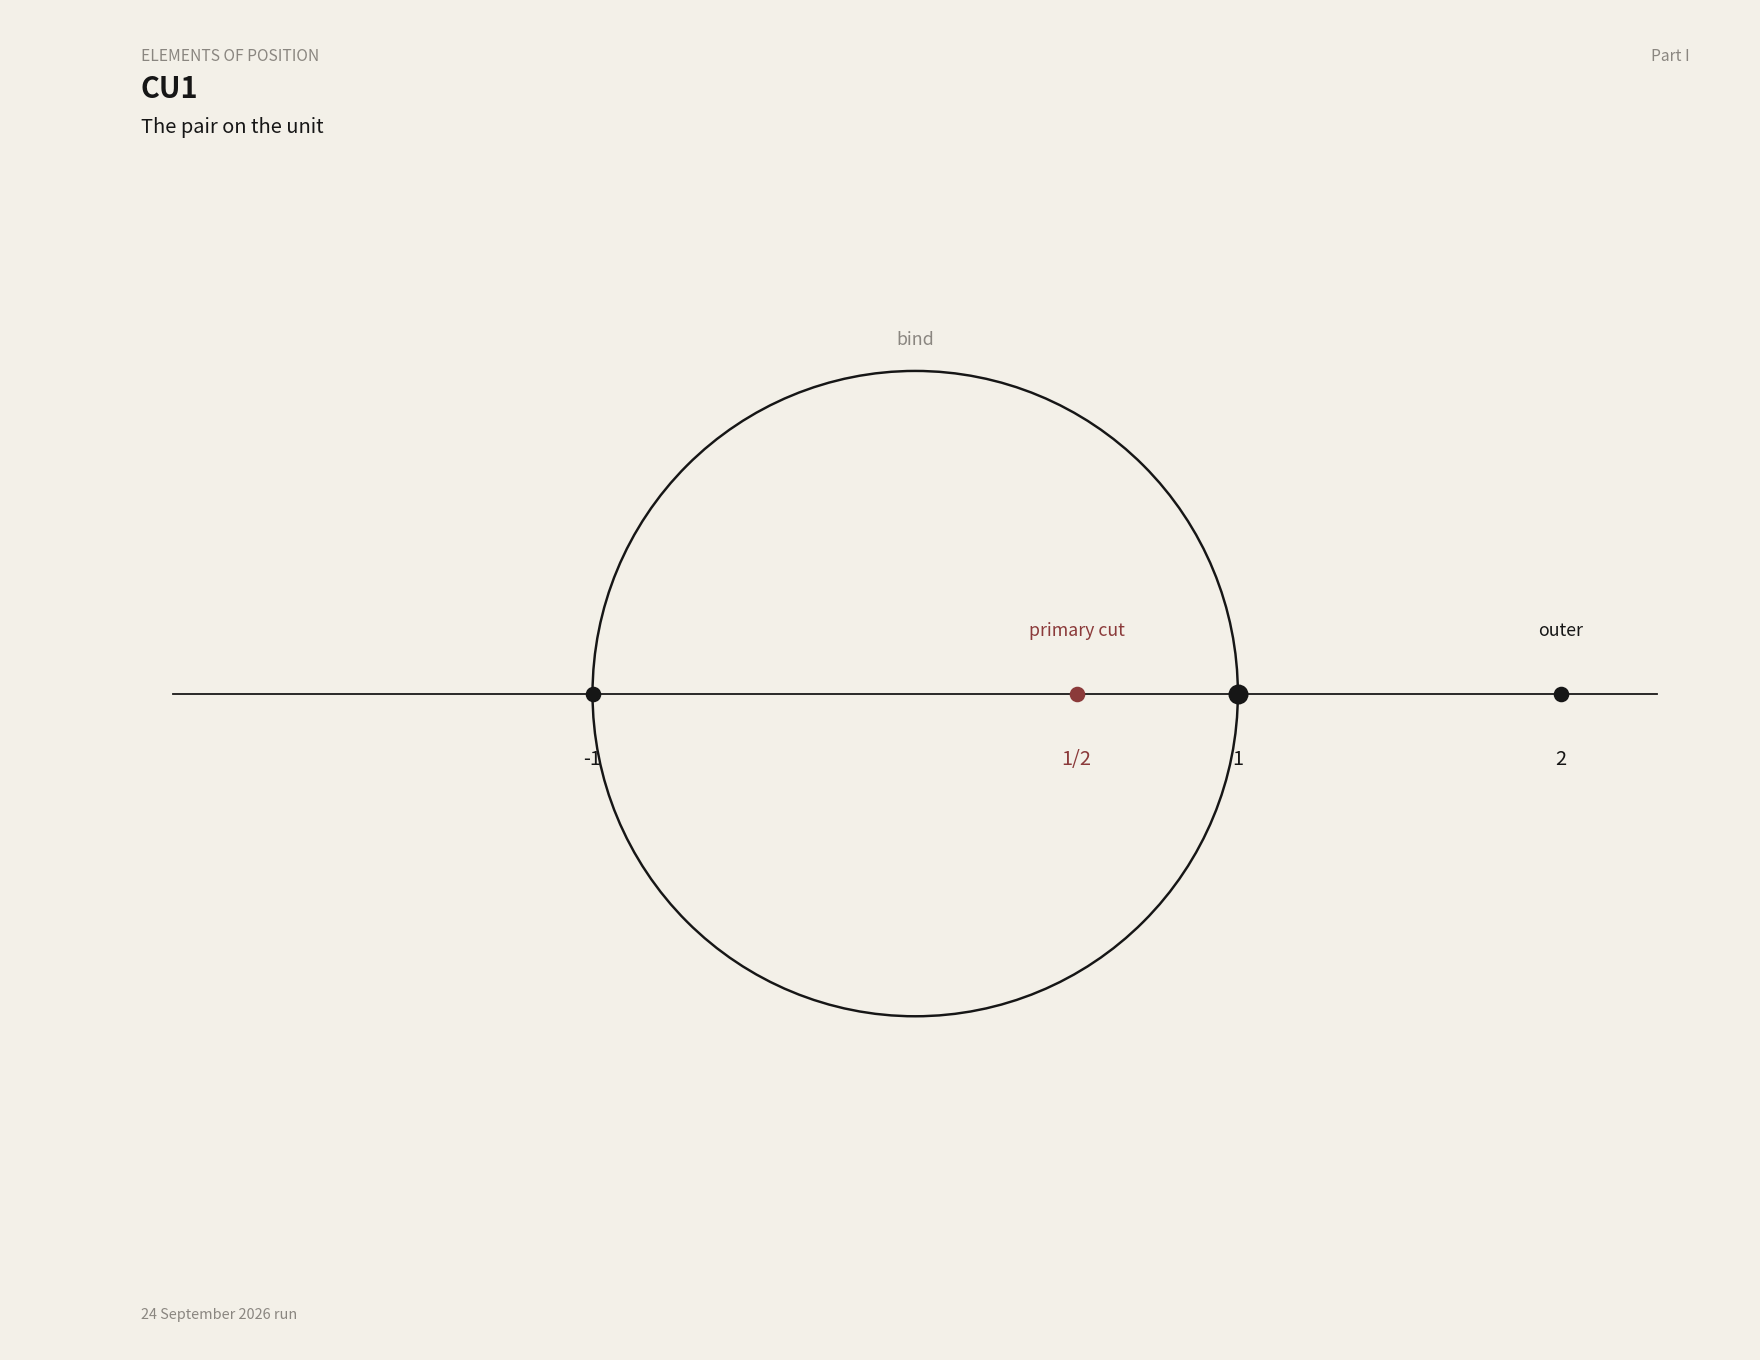
\includegraphics[width=0.92\textwidth]{CU1_pair.png}
\caption{Sheet CU1. The bind, the primary cut, the pair on the line. The lock is where $n=1/n$.}
\end{figure}

Nothing after the lock is a new kind of figure.
Every later \(n\) writes the same pair, the same product, the same leftover, at a larger \(r\).

This arithmetic does not require a walker.
It is true of the integer whether or not any heading ever moved.
The live kernels of this series both compute it: \(\mathtt{pair}(m)\) in the walk kernel, \(\mathtt{ring}(n)\) in the n-gon kernel.
Two routes, one pair.

\section{What the literature already holds}

AM--GM for two terms is the geometric-mean theorem wearing an inequality.
Inversion in a circle, \(r\mapsto 1/r\) on the unit, is classical.
The pair \((n,1/n)\) is that transformation on the ray.

Archimedes sandwiches a circle between inscribed and circumscribed regular polygons.
The present work does not continue that count in order to squeeze a decimal for \(\pi\).
It stops the count in order to keep the close visible as an integer and the inverse parts visible as a pair whose product is \(1\).

Almost nothing proved in this part is new.
What is offered is the joint those facts already share, named as a lock, and not used as a discovery of constants.

\section{The integer close}

A circle is asked only when one asks a different elementary question: if the diameter is exactly \(1\), when does the figure close?
The answer is an integer --- the same \(1\).

The later integers repeat that close.
At finished count \(n\) the local circle has diameter \(n\) and radius \(n/2\).
That convention is the n-gon kernel's only placement rule.
It is also the radius the continuous-clock reading writes as \(k/2\) when scale \(k\) is the walk's own half-turn count.
Those readings are later.
They do not revise the pair.

\section{What stands}

Forced:
the unit as a finished hold whose interior does not finish;
AM--GM, with equality only at an even split;
the primary cut \(1/2\);
the pair \((n,1/n)\), product \(1\), geometric mean \(1\);
the leftover \(\tau(n)=(n-1)^2/(2n)\), zero only at the lock;
inversion as the map that writes the pair.

Not granted:
an angle inside a step;
a residual;
a second generator;
a value of \(\pi\) treated as reached at a finite mark.

Where is \(1\)?
It is the lock.
The trace of that lock --- two moves, a heading, a count of crossings --- is the next part.

\end{document}
